\documentclass{itatnew}
   \lstdefinestyle{mystyle}{
        language=python,
    basicstyle=\fontencoding{T1}\footnotesize\fontfamily{lmtt}\fontseries{c}\selectfont,
        keepspaces=true,
    }
    \lstset{style=mystyle}

%% !!!dolezite: ak pisete po slovensky alebo po cesky pouzite
%% \documentclass[slovensky]{itatnew}
%% \documentclass[cesky]{itatnew}
\usepackage[dvipsnames]{xcolor}
\usepackage{listings}
\usepackage{minted}
\usemintedstyle{vs}

\makeatletter
\def\blfootnote{\xdef\@thefnmark{}\@footnotetext}
\makeatother

\begin{document}

\title{confr - A Configuration System for Machine Learning Projects}

\author{Mattias Arro\inst{1}}

\institute{
\email{mattias.arro@gmail.com},\\
\texttt{www.uxo.ai}
}

\maketitle              % typeset the title of the contribution
\blfootnote{Copyright \copyright 2022 for this paper by its author. Use permitted under Creative Commons License Attribution 4.0 International (CC BY 4.0).}

\begin{abstract}
Finding a performant machine learning model usually requires exploring different combinations of model hyperparameters, preprocessing steps, data generation and train logic.
To facilitate a clear analysis of the factors that determine accuracy, it is useful to make the data processing and train pipeline highly configurable such that a combination of a code version and configuration file uniquely determins the behaviour of the system.
A poor configuration system can lead to repetitive code that is hard to maintain, understand, and brittle due to insufficient configuration validation logic. This paper outlines the design and usage of confr, a concise and flexible configuration system geared towards Python-based machine learning projects. It combines some of the capabilities of commonly used systems (such as gin-config, OmegaConf, and Hydra) into a library which aims to reduce repetitive code and maintenance overhead. It can be used both as part of a notebook-based and script-based workloads, and can be used for ensuring that there is no accidental difference between inference-time and train-time behaviour.
\end{abstract}


\section{Introduction}

The goal of machine learning (ML) practitioners is to find a "good model".
This is broadly determined by three factors: (training and validation) data, code (preprocessing, model implementation, train loop), and hyperparameters (configuration).
By hyperparameters we mean any non-learnable parameter/configuration that influences how the code gets executed, which may be in the data processing, model intialisation or inference, or train loop.
When running experiments, exact and immutable versions of the three should always be stored, so that we can (1) analyse the factors that influence accuracy and (2) reproduce the results of an earlier experiment.

Early in developing a ML system, code tends to hardcode most choices for data processing, model implementation and hyperparameters.
Experimentation in this setting would require changes to the code, which means that to compare two experiments one needs to find the differences of code used in each train run, or rely on the experimenter's description of the hypothesis that was tested.
Given that most ML experiments are done in notebooks where comparing code with version control is difficult, comparing large numbers of such experiments is not feasible.

A better approach is to make the code highly configurable, so that alternative behaviours can be achieved by using different hyperparameter values.
Now triggering many train runs (on the same code and data version) creates a dataset of hyperparameter sets and corresponding evaluation metrics.
The relationship between hyperparameters and metrics can be analysed for insights that inform future hyperparameter choices or code changes.
A highly configurable train pipeline also lends itself for automatic model tuning approaches such as brute-force grid/random search, or methods like Bayesian optimisation that use ML to find values for hyperparameters which maximise validation accuracy.

There are many ways to make a system configurable, such as creating an ad hoc solution from scratch or using a 3rd party config\footnote{We use the words "config" and "configuration" interchangeably, as is common in industry.} system.
The following is a list of qualities we would expect from a config system, which we will later use to evaluate our proposed system confr against alternatives.

\begin{enumerate}
    \item \textbf{Minimise boilerplate code.} There should not be much repetitive code to have a highly configurable system.
    \item \textbf{Minimise repetitive config.} There should be ways to reuse, rather than repeat, individual config values.
    \item \textbf{Composability of config objects.} It should be possible to reuse and compose different configurations, which is crucial for large systems.
    \item \textbf{Low maintenance overhead.} A config system should reduce (rather than add to) the difficulty of refactoring and developing the code base.
    \item \textbf{Low cognitive load.} A config system should make it easy to understand which variables are configurable and where that configuration comes from. It is highly related (but not fully determined) by the following three qualities.
    \item \textbf{Clearly identifyable configurable arguments.} It should be clear just by looking at a function if its argument is a configurable hyperparameter. This improves readability and decreases the chance of accidentally forgetting to provide a config value.
    \item \textbf{Consistent mapping between config keys and variables / arguments.} The system should encourage a one-to-one mapping between keys\footnote{Configuration files are (possibly nested) key-value pairs. We call the names of configurable hyperparameters as "config keys".} in the config file and configurable arguments. Such mapping alleviates the cognitive load in translating differences between config keys and variable names, and makes it easy to search for all places where a config key is used.
    \item \textbf{Global config values.} In most cases we expect the value of a config key to be the same across the code base, and a config system should encourage this. For example, if a preprocessing function assumes \mintinline{Python}{max_img_dimensions = (128, 128)}, then so should the function which builds the neural network whose input tensor would have the shape \mintinline{Python}{(128, 128, 3)} - otherwise the model's input dimensions would be incompatible with the images created by the preprocessor.
    \item \textbf{Centralised, multi-key validation of config.} Validation of config values should be centralised in a single place, rather than scattered around the project in an ad hoc manner. This (1) ensures we fail quickly with a helpful message when reading a faulty config (rather than waiting for the relevant code path to be reached, which may happen at a much later state), and (2) allows defining validation logic that sets constraints on several config keys simultaneously.
    \item \textbf{Usable in a notebook as well as CLI.} The system should be easy to use in an exploratory notebook-based setting, where one might want to dynamically (re-)define and access config values, and to ultimately write the current active configuration to a file. It should also work in a script-oriented CLI\footnote{CLI - Command Line Interface} setting, where main configuration is loaded from a file, and certain config values or whole sections can be overridden via command line arguments.
    \item \textbf{Configurable Python references and singletons.} It should be possible to refer to Python objects (functions, classes, constants, objects) and create global singletons from callable references (functions, classes).
\end{enumerate}


\section{Related Work}

In this section we provide a brief overview of existing configuration systems.
We first describe what typical ad hoc solutions look like, and then look at three config systems which are commonly used\footnote{By "commonly used" we mean systems we were able to find by doing relevant Google searches, reading relevant discussion threads, and looking at GitHub activity for these projects.} for ML workloads: OmegaConf \cite{OmegaConf}, gin-config \cite{gin-config}, and Hydra \cite{hydra}.
gin-config is explicitly designed for ML work, while OmegaConf and Hydra are generic config systems.

\subsection{Ad Hoc Systems}

Machine learning projects that do not use a specialised config system tend to consist of Python scripts where hyperparameters are defined as command line arguments.
Libraries like argparse\footnote{https://docs.python.org/3/library/argparse.html} and click\footnote{https://click.palletsprojects.com/} can be used for easier parsing of command line arguments or providing arguments via environment variables.
The individual config values get passed to downstream functions where necessary.

Alternatively, a regular Python dictionary containing the configuration might be read from a YAML/JSON file, and passed along to functions that depend on it.
Either the full configuration object or individual config values might be passed along, depending on programming style.
It is generally not easy to unify such CLI-based and file-based configuration styles without using a specialised config system.


\subsection{OmegaConf}

OmegaConf builds on YAML file format, and adds a powerful interpolation mechanism, which enables accessing config keys from other parts of the file. The below example shows both absolute (\mintinline{Python}{${server.host}$}) and relative (\mintinline{Python}{${.url}$}) references to other parts of the config file.

\begin{figure}[H]
    \centering
    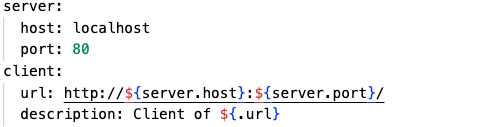
\includegraphics[width=8cm]{o1.png}
\end{figure}

OmegaConf configursation is represented as a Python object, which can be accessed as a nested object or dictionary:

\begin{figure}[H]
    \centering
    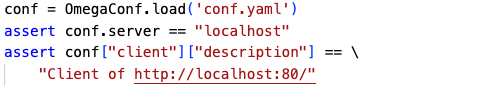
\includegraphics[width=8cm]{o2.png}
\end{figure}

\subsection{gin-config}
gin-config makes use of \mintinline{Python}{@gin.configurable} decorators around function and class definitions. For functions (and initialisers of classes) decorated like this, arguments are substituted from the global config which is initialised with \mintinline{Python}{gin.parse_config_file("conf.gin")}. Attributes with default value of \mintinline{Python}{gin.CONFIGURED} need to have a config specified in the .gin config file; other arguments can (but do not have to be) configured with gin.

\begin{figure}[H]
    \centering
    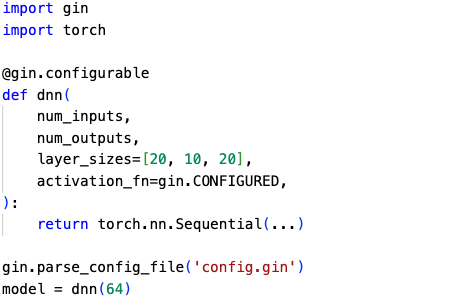
\includegraphics[width=8cm]{g1.png}
\end{figure}

The config file is a custom text format, which is a simplified subset of Python.
Using \mintinline{Python}{dnn.num_outputs = 10} would ensure all functions named \mintinline{Python}{dnn} will have the value of \mintinline{Python}{num_outputs} substituted as \mintinline{Python}{10}.
Using \mintinline{Python}{path.to.mymodule.dnn.num_outputs = 10} would ensure it happens only to the function in the \mintinline{Python}{path.to.mymodule} module.
As special syntax, values that start with "@" refer to other gin-configurable functions or classes; values that start with "@" and end with "()" first get called before being passed as arguments.

\begin{figure}[H]
    \centering
    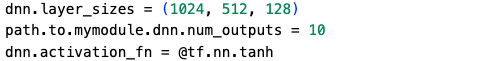
\includegraphics[width=8cm]{g2.png}
\end{figure}

\subsection{Hydra}

Hydra is a feature-rich config system. The entrypoint function of the program using Hydra should be annotated with a \mintinline{Python}{@hydra.main} decorator, which defines the directory where config files are stored, and config name (filename without the .yaml extension in the directory). When called, the function receives an OmegaConf cfg object as an argument, which can be passed to downstream functions. Therefore the config files support all the syntax and functionality of OmegaConf, and some features that Hydra adds. For detailed examples, refer to Hydra documention\footnote{https://hydra.cc/docs/intro/}.

\begin{figure}[H]
    \centering
    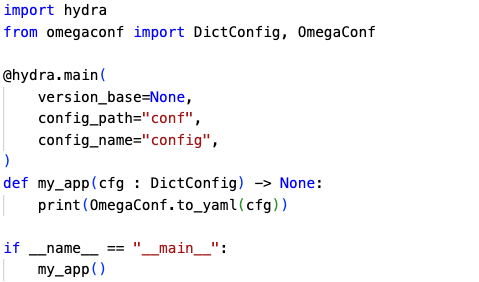
\includegraphics[width=8cm]{h.png}
\end{figure}


\section{Overview of confr}

In this section, we show the basics of how to use confr. For complete and up-to-date documentation see https://github.com/mattiasarro/confr.

\subsection{Basic Usage}

In confr, configs are initialised similarly to gin-config: functions and classes can be decorated with \mintinline{Python}{confr.bind}, which ensures that function and class initialiser arguments will be substituted from the currently active config. The following example shows a function that expects at least the \mintinline{Python}{num_outputs} key (and optionally \mintinline{Python}{layer_sizes}) to be defined in conf/base.yaml. Before calling any confr-configured functions, \mintinline{Python}{confr.init} must be called, which creates an implicit global config object.

\begin{figure}[H]
    \centering
    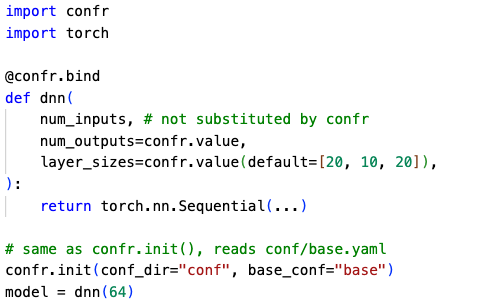
\includegraphics[width=8cm]{c1.png}
\end{figure}

All config files use the special form of YAML used by OmegaConf (with a few special cases described in the next subsections). In the default case, the arguments get bound to top-level config keys of the same name in the YAML file. So in the above example, our \mintinline{Python}{conf/base.yaml} could look like this:

\begin{figure}[H]
    \centering
    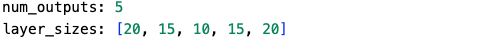
\includegraphics[width=8cm]{c2.png}
\end{figure}

\subsection{Custom Config Key to Argument Mapping}

In some cases, a one-to-one mapping of config keys to function argument names can be limiting, so we offer two ways to customise this. Assume we have the following config:

\begin{figure}[H]
    \centering
    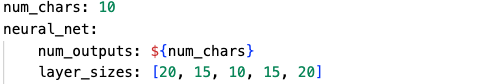
\includegraphics[width=8cm]{c3.png}
\end{figure}

When wrapping a function with \mintinline{Python}{confr.bind}, we could tell it to only map keys under the \mintinline{Python}{neural_net} config key:

\begin{figure}[H]
    \centering
    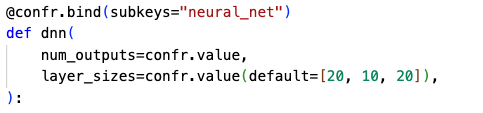
\includegraphics[width=8cm]{c4.png}
\end{figure}

The other option is to pass the full path in the config to \mintinline{Python}{confr.value}:

\begin{figure}[H]
    \centering
    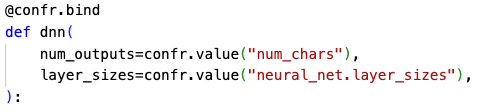
\includegraphics[width=8cm]{c5.png}
\end{figure}


\subsection{Python References and Singletons}

confr adds special syntax to the YAML format supported by OmgaConf, which can be used to load Python object or initialise global singletons. Config values which start with a "@" are "\textbf{Python references}"\footnote{References to Python objects and references to other config values in the file look quite similar, since they both use dot notation. Python references start with a "@", and they refer Python modules like in absolute imports (which usually correspond to folder structure). Referencing other parts of a config file start with a "\$" and refer to the "path" in the YAML file, which follows the nesting of config keys.}. A common use for this is to make a preprocessing or augmentation function as a configurable argument, so that you can try out different preprocessors without changing the code. For example:

\begin{figure}[H]
    \centering
    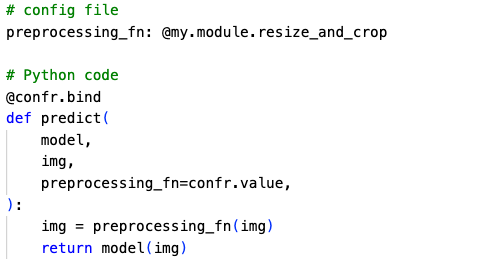
\includegraphics[width=8cm]{c6.png}
\end{figure}

When \mintinline{Python}{predict} is called, the Python module \mintinline{Python}{my.module} is imported and the \mintinline{Python}{resize_and_crop} attribute is read from it. Any Python object could be referenced in config files - function, class, variable, constant - as long as its module is available on PYTHONPATH, which usually includes all modules in the project root as well as installed libraries such as tensorflow.

Config values which start with a "@" and end with "\mintinline{Python}{()}" are \textbf{singletons} - Python references which get called before becoming part of the current active config and being passed as keyword arguments. For example you might define an \mintinline{Python}{encoder: @my.module.my_encoder()} key-value pair in the config. Now if a function defines an argument as \mintinline{Python}{encoder=confr.value}, then \mintinline{Python}{@my.module} gets imported and its \mintinline{Python}{my_encoder()} callable gets called before being passed as the argument value. Once \mintinline{Python}{my_encoder()} is called, its return value gets memoized and any subsequent functions which use the \mintinline{Python}{encoder} config will receive the same, pre-initialised object. Singletons can be referenced in other parts of the config using the familiar OmegaConf format of \mintinline{Python}{${config_key.subkey.singleton}$}.

Note that \mintinline{Python}{my_model1} and \mintinline{Python}{my_model2} in the following listing are the same object.

\begin{figure}[H]
    \centering
    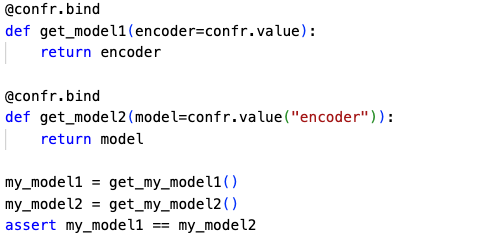
\includegraphics[width=8cm]{c7.png}
\end{figure}


\subsection{Scoped Arguments in Singletons}

If you would like to configure input arguments specifically for singletons, you can do the following:

\begin{figure}[H]
    \centering
    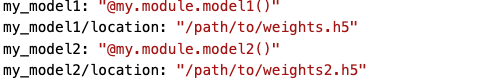
\includegraphics[width=8cm]{c8.png}
\end{figure}

Now \mintinline{Python}{my_model1} singleton will be initialized with \mintinline{Python}{location="/path/to/weights.h5"} and \mintinline{Python}{my_model2} singleton will be initialized with \mintinline{Python}{location="/path/to/weights2.h5"}. This way they can both define an input argument called location and still receive a unique value at initialization time. We call \mintinline{Python}{my_model1/location} as a scoped argument, i.e. the value of location is present in only the \mintinline{Python}{my_model1} singleton scope.

Note that you can still use the regular, non-scoped arguments along with scoped ones. For example, both \mintinline{Python}{my_model1} and \mintinline{Python}{my_model2} might define \mintinline{Python}{img_h=confr.value}, and this value will be the same when initializing both singletons.

\subsection{Call-time Overrides}

When running a Python program configured with confr, individual values can be overriden in two ways:

\begin{enumerate}
    \item Passing command-line arguments such as \mintinline{Python}{--key1.subkey1=value}.
    \item Setting environment variables such as \mintinline{Python}{confr__key1__subkey1=value}.
\end{enumerate}

\subsection{Run-time overrides}

When working in a notebook, modifying the YAML file to change the active config is cumbersome.
You could instead initialize the config at the start of the notebook by selectively providing overrides to the keys you care about like this:

\begin{figure}[H]
    \centering
    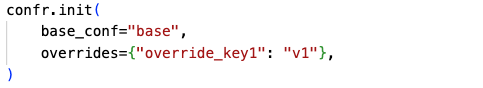
\includegraphics[width=8cm]{c9.png}
\end{figure}

If you do not want to re-initialise the whole config, but would like to set individual config values, use \mintinline{Python}{confr.set("my_key", value)}. Doing this would not re-initialise other config keys or singletons that may depend on \mintinline{Python}{my_key}.

You may also want to provide overrides to config values temporarily, for the duration of calling a function (and any downstream functions called by this function). For example, you might want to iterate over a list of \mintinline{Python}{p_thresh} values and calculate accuracy for each \mintinline{Python}{p_thresh}.

Our first attempt at solving this would look like this:

\begin{figure}[H]
    \centering
    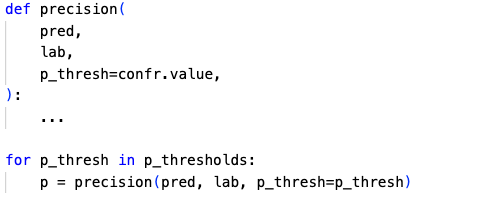
\includegraphics[width=8cm]{c10.png}
\end{figure}

This would work if \mintinline{Python}{precision} is the only place that uses the \mintinline{Python}{p_thresh} that is passed in. But if \mintinline{Python}{precision} calls \mintinline{Python}{sub_function} whose \mintinline{Python}{p_thresh} value comes from confr, then the value of \mintinline{Python}{p_thresh} in \mintinline{Python}{sub_function} will be the same as in the config file and not the one we passed to \mintinline{Python}{precision}. What we need here is to temporarily set the value of \mintinline{Python}{p_thresh} config key in the whole confr, like this:

\begin{figure}[H]
    \centering
    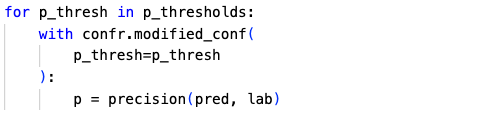
\includegraphics[width=8cm]{c11.png}
\end{figure}

\subsection{Config Spanning Multiple Files}

Suppose you have the following config files:

\begin{figure}[H]
    \centering
    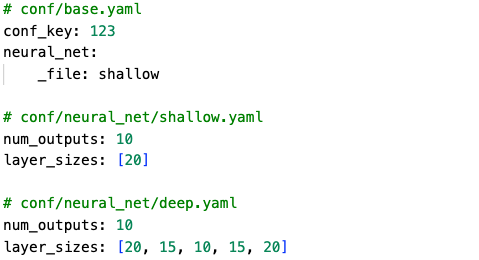
\includegraphics[width=8cm]{c12.png}
\end{figure}

Once the config is loaded, the effective final config would look like  this, because the \mintinline{Python}{_file} special key tells confr to take the configuration for \mintinline{Python}{neural_net} subkeys from another file.

\begin{figure}[H]
    \centering
    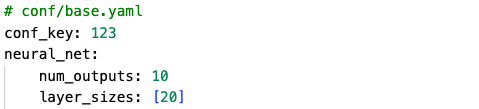
\includegraphics[width=8cm]{c13.png}
\end{figure}

But you could also override which neural net config gets used, by passing \mintinline{Python}{--neural_net._file=deep} when running the program. Note that there is a convention between the config keys and the folders from where \mintinline{Python}{_file} references are searched.

\subsection{Accessing the Active Config}

Sometimes we need to explicitly fetch the value of a key in our config system. You can use \mintinline{Python}{confr.get} and \mintinline{Python}{confr.set} accessors to modify the current active conf:

\begin{figure}[H]
    \centering
    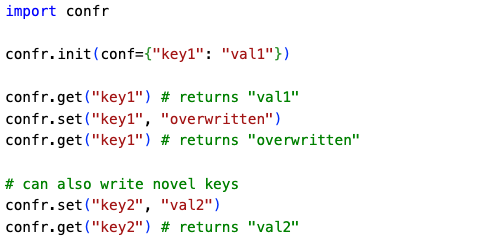
\includegraphics[width=8cm]{c14.png}
\end{figure}

You can also save the current active config as a YAML file, for example at the end of training.
The code for training the model and doing inference should be in the same version control project; train-time and inference-time pre-processing should be handled by the same function(s).
This way, if code for inference is initialised from the same code revision and active config that was used during training, there would be no accidental difference between train time and test time behaviour.

\begin{figure}[H]
    \centering
    
\includegraphics[width=8cm]{c15.png}
\end{figure}

\subsection{Validation}

Two types of validations can be done with confr. Each config file with name \mintinline{Python}{filename.yaml} can have an optional \mintinline{Python}{filename_types.yaml} counterpart, which defines the datatype of all (or a subset of) the config keys. Currently, only primitive Python types are supported, but more complex solutions will be added.

For example:

\begin{figure}[H]
    \centering
    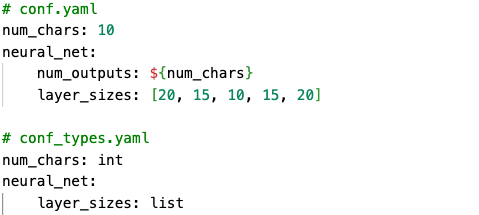
\includegraphics[width=8cm]{c16.png}
\end{figure}

However, once the config gets complex enough, there is a need to validate different combinations of config values. For example, imagine we have the following config, which states that 50\% of the samples come from labelled dataset, 25\% come from data generator 1 and 25\% come from generator 2:

\begin{figure}[H]
    \centering
    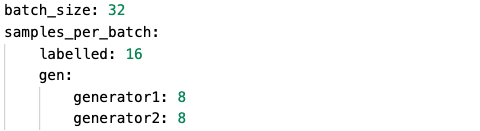
\includegraphics[width=8cm]{c17.png}
\end{figure}

In confr we can define a validator that ensures that everything in \mintinline{Python}{samples_per_batch} sums to \mintinline{Python}{batch_size}.

\begin{figure}[H]
    \centering
    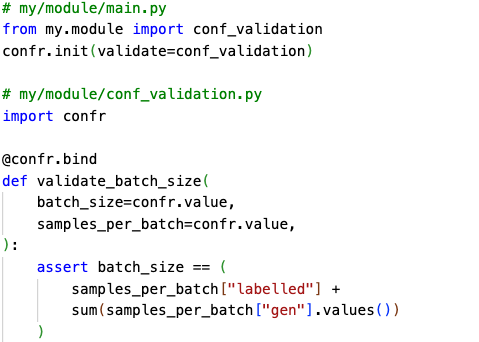
\includegraphics[width=8cm]{c18.png}
\end{figure}


\section{Evaluation}

We will now evaluate the competing systems and confr on the desired qualities outlined in the introduction, giving each a somewhat subjective \textcolor{Maroon}{BAD} / \textcolor{YellowOrange}{OK} / \textcolor{OliveGreen}{GOOD} mark.

\begin{enumerate}
    \item \textbf{Minimise boilerplate code.}
        \begin{itemize}
            \item \textcolor{Maroon}{BAD}: ad hoc, OmegaConf. Passing down configuration dictionaries or individual config values can be very verbose. So can be setting up CLI arguments in ad hoc systems.
            \item \textcolor{YellowOrange}{OK}: Hydra. Different functions can request a config object, and read individual keys from it. However generally there is a single config object that gets passed along.
            \item \textcolor{OliveGreen}{GOOD}: gin, confr. Configurable function arguments receive a value directly from the config system, which is most concise.
        \end{itemize}
    \item \textbf{Minimise repetitive config.}
        \begin{itemize}
            \item \textcolor{Maroon}{BAD}: ad hoc. No way to reuse / refer to other values in YAML/JSON files.
            \item \textcolor{YellowOrange}{OK}: gin-config. It is possible to reuse values, but in a cumbersome way, and the config file format is somewhat verbose (since all occurences of a config value need to be listed).
            \item \textcolor{OliveGreen}{GOOD}: OmegaConf, Hydra, confr. It is possible to reuse values and create concise config files.
        \end{itemize}
    \item \textbf{Composability of config objects.}
        \begin{itemize}
            \item \textcolor{Maroon}{BAD}: ad hoc, OmegaConf, gin-config. Not supported.
            \item \textcolor{OliveGreen}{GOOD}: Hydra, confr. Supported.
        \end{itemize}
    \item \textbf{Low maintenance overhead.}
        \begin{itemize}
            \item \textcolor{Maroon}{BAD}: ad hoc, gin-config. Passing along config objects/values slows down refactoring. gin-config also often requires config changes when the relevant code changes (renaming/moving functions). Ad hoc systems might need to maintain CLI argument lists.
            \item \textcolor{YellowOrange}{OK}: OmegaConf, Hydra. Moving code around requires changes to passing of config values, but this is less troublesome than changes required by gin-config or maintaining CLI argument lists in ad hoc systems.
            \item \textcolor{OliveGreen}{GOOD}: confr. Config files and other parts of the source generally do not need to be changed on renaming or moving functions, because the config file makes no assumptions about where the config is used and config values do not need to be propagated.
        \end{itemize}
    \item \textbf{Low cognitive load.}
        \begin{itemize}
            \item \textcolor{Maroon}{BAD}: gin-config, Hydra. It is not clear, without reading the configuration file and upstream code carefully, which arguments are configured and where the value comes from.
            \item \textcolor{YellowOrange}{OK}: ad hoc, OmegaConf, confr.
            The initial cognitive load of understanding how a configurarion is loaded in ad hoc systems and OmegaConf is low (for example, it's easy to understand what reading a YAML file or using argparse does). However it is much harder to reason about how the whole system behaves due to the next three qualities.
            In confr, it takes more effort to think about many possible places where configurations can come from (multiple files, command line overrides), but it is easier to reason about the whole system due to the following three qualities.
        \end{itemize}
    \item \textbf{Clearly identifyable configurable arguments.}
        \begin{itemize}
            \item \textcolor{Maroon}{BAD}: ad hoc, OmegaConf, Hydra. When reading code (that is "far away" from the part that initialises config), it is not clear which arguments are configurable.
            \item \textcolor{YellowOrange}{OK}: gin-config. It is possible to make it explicit that some arguments should receive a value from configuration, but this is not a requirement.
            \item \textcolor{OliveGreen}{GOOD}: confr. It is intentionally not possible to configure an argument in confr without making it explicit in code that the value is configurable.
        \end{itemize}
    \item \textbf{Consistent mapping between config keys and variables / arguments.}
        \begin{itemize}
            \item \textcolor{Maroon}{BAD}: ad hoc, OmegaConf, gin-config, Hydra. In all these systems such consistency is not encouraged, which makes it harder to read, understand and refactor.
            \item \textcolor{YellowOrange}{OK}: confr. Such consistency is enforced by default, though in rare cases it is possible to bypass this (for example when you need to use an externally-provided config file).
        \end{itemize}
    \item \textbf{Global config values.}
        \begin{itemize}
            \item \textcolor{Maroon}{BAD}: ad hoc, OmegaConf, Hydra. It is easy to have multiple configuration objects, or to have a different value in different places for the same config key.
            \item \textcolor{OliveGreen}{GOOD}: gin-config, confr. There can be only one globally active configuration. In confr, each config key always has the same value.
        \end{itemize}
    \item \textbf{Centralised, multi-key validation of config.}
        \begin{itemize}
            \item \textcolor{Maroon}{BAD}: gin-config. No validation system provided, hard to add one.
            \item \textcolor{YellowOrange}{OK}: ad hoc, OmegaConf, Hydra. Centralised validation system can be added through user code to OmegaConf or file-based ad hoc systems, though this is harder to do in CLI-based ad hoc systems in a concise way. Hydra has a validation system, but this is mostly limited to data type based checks, which are insufficient.
            \item \textcolor{OliveGreen}{GOOD}: confr. Supported, built in.
        \end{itemize}
    \item \textbf{Usable in a notebook as well as CLI.}
        \begin{itemize}
            \item \textcolor{Maroon}{BAD}: ad hoc, gin-config. Ad hoc systems tend to work well either for notebook-based approaches (e.g. reading a global YAML file as a config dict), or work as a sophisticated CLI script, but not both. There is no support to override options from the CLI in OmegaConf and gin-config.
            \item \textcolor{OliveGreen}{GOOD}: OmegaConf, Hydra, confr. Can be used in both settings.
        \end{itemize}
    \item \textbf{Configurable Python references and singletons.}
        \begin{itemize}
            \item \textcolor{Maroon}{BAD}: ad hoc. Usually not supported.
            \item \textcolor{YellowOrange}{OK}: OmegaConf, Hydra. Supported, but cumbersome to use.
            \item \textcolor{OliveGreen}{GOOD}: gin-config, confr. Supported, easy to use.
        \end{itemize}
\end{enumerate}


The results are summarised in the following table.
From it we can see that confr exhibits the good qualities of Hydra and gin-config, while alleviating some of the downsides one or the other.
This is not a coincidence, since confr was in many ways inspired by these two, though the exact way confr achieves these qualities may be different.

\begin{figure}[H]
    \centering
    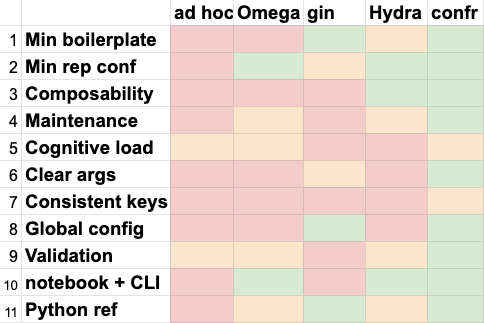
\includegraphics[width=8cm]{eval.png}
\end{figure}

There are features not supported by confr which other libraries provide that will be added in later versions: tab completion and more detailed type checking provided by Hydra. Hydra also has some features that were intentionally not made part of confr, such as multi-run options, custom working dir and logger config, since these were not considered relevant with respect to the evalation criteria, which we considered most useful for a ML-oriented config system.


\begin{thebibliography}{5}

\bibitem {gin-config}
Holtmann-Rice, D., Guadarrama, S., Silberman, N.:
Gin Config.
https://github.com/google/gin-config (2018)

\bibitem {OmegaConf}
OmegaConf.
https://github.com/omry/omegaconf (2012)

\bibitem {hydra}
Yadan, E.:
Hydra - A framework for elegantly configuring complex applications,
https://github.com/facebookresearch/hydra (2019)

\end{thebibliography}
\end{document}
